%%%%%%%%%%%%%%%%%%%%%%%%%%%%%%%%%%%%%%%%%%%%%%%%%%%%%%%%%%%%%%%%%%%%%%%%%%%%%%%%
%%%%%%%%%%%%%%%%%%%%%%%%%%%%%%%%%%%%%%%%%%%%%%%%%%%%%%%%%%%%%%%%%%%%%%%%%%%%%%%%
%%%%%%%%%%%%%%%%%%%%%%%%%%%%%%%%%%%%%%%%%%%%%%%%%%%%%%%%%%%%%%%%%%%%%%%%%%%%%%%%
Este capítulo descreve com detalhes o ambiente de desenvolvimento que foi realizado neste projeto.

\section{Ambiente proposto}%

	O desenvolvimento do ambiente foi realizado para a plataforma web. Consiste em três partes principais:
	
	\begin{itemize}
		\item Editor de texto
		\item Montador
		\item Simulador
	\end{itemize}

	Toda a parte de interação com o usuário utiliza as tecnologias web: \textit{javascript}, para ter uma interface dinâmica, utilizando a biblioteca \textit{jQuery}. Para a estruturação utilizou-se a linguagem de marcação \textit{HTML}, e a folha de estilos \textit{CSS} para formatação do layout.

	Apesar de ter sido desenvolvido para rodar na web, os componentes "Montador" e "Simulador", podem ser utilizados separados, por exemplo em linha de comando. Basta ter instalado um interpretador \textit{Python 3.x}


\section{Arquitetura de software}

	Como na maioria das aplicações web, utilizamos o modelo Cliente-Servidor, como ilustrado anteriormente na figura \ref{fig:client-server-model}. Neste modelo, o usuário é um cliente, que faz requisições ao servidor através da internet. 

	Usuário faz requisição da página inicial, onde ele pode escrever seu código, então a partir disso ele irá enviar este código para o servidor, requisitando a montagem, e então receberá a saída do montador, ou a mensagem apropriada no caso de erros.

	Com o código montado, pode se salvar em arquivos os dados da montagem em diferentes formatos, binário, hexadecimal ou em formato \textit{MIF ("Memory Initialization File")}, utilizado para inicializar memórias em FPGA's da Altera. Esses dados podem ser enviados novamente para o servidor em uma nova requisição de simulação, e então o servidor irá responder os resultados do programa, qual o estado de memória final, valores dos registradores e, se houver, mensagens de saída.

	Para melhorar a interação do usuário com a ferramenta, foi utilizado a metodologia de \textit{Single Page Application}~\cite{mikowski2013single}. Desta maneira, utilizamos apenas uma página e carregamos conteúdos dinâmicamente na mesma página.

	Para a implementação da metodologia foi utilizado a biblioteca \textit{jQuery}. Existem tecnologias mais modernas mais apropriadas para a implementação de uma SPA, porém foi decido não utilizá-las por questões de tempo para a aprendizagem destas.

	O código \textit{jQuery} faz chamadas HTTP assíncronas ao \textit{back-end} usando os métodos POST e GET ao pressionar algum botão de ação do sistema. 

	Abaixo iremos descrever por módulos cada componente do sistema.
	
	\subsection{\textit{front-end}}
	
		O \textit{front-end} da aplicação como já explanado anteriormente é a parte visual da aplicação. É a parte do software que lidará diretamente com a usabilidade e experiência do usuário. Nesta seção será abordado como foi implementado com maiores detalhes dentro da solução apresentada neste projeto.

		\subsubsection{Single Page Application}
		
			Single Page Application é uma única página com todos os componentes carregados, porém escondidos. Com isso evitamos recarregar a página várias vezes, pois a quantidade de dados que teríamos que  enviar e receber do servidor web seria alta, além de termos que processar esses dados para manter o estado atual do sistema sempre sincronizado.

			Na parte de \textit{front-end} temos três módulos ou seções. Estes módulos são definidos por uma estrutura em HTML utilizando a \textit{tag section} com ID's. Desse jeito podemos separar visualmente com CSS e funcionalmente com \textit{javascript}. As seções existentes são entrada, saída e simulator.

			Cada seção pode ser acessada pelo menu global da aplicação como mostrado na figura \ref{fig:menu_global}.

			\begin{figure}[h!]
			  \centering
			  
\includegraphics[width=4cm]{img/menu_global.png}
			  \caption{Menu global do sistema. Principal componente de navegação.}
			  \label{fig:menu_global}
			\end{figure}

			Neste menu vemos duas partes separadas por uma linha horizontal, a parte superior contém as seções do sistema, enquanto a parte inferior contém seções de informações.

			Para a lógica do \textit{front-end} temos dois módulos em \textit{jQuery}, o \textit{riscv\textunderscore flow} e \textit{riscv\textunderscore functions}. Detalharemos estes módulos abaixo.

			\subparagraph{riscv\textunderscore flow}

				Este módulo trata de associar eventos aos botões do sistema para esconder e mostrar seções através de alterações no CSS. E também associa os botões de ações do sistema.

				Por exemplo, para mostrarmos a seção de simulação, escondemos a seção de entrada e a seção de saída e mostramos a seção de simulação, e então para mostrar outra seção mostramos essa seção e escondemos a de simulação.

				A associação dos eventos de comunicação com o \textit{back-end} também é feito no \textit{riscv\textunderscore flow}.

				Por exemplo, ao clicarmos no botão de montagem, a função que associa o clique no botão com a funcionalidade de montagem é escrita aqui. Porém a funcionalidade da comunicação em é feita no módulo \textit{riscv\textunderscore functions}, que iremos detalhar no próximo parágrafo.  

			\subparagraph{riscv\textunderscore functions}

				São implementadas as funcionalidades e eventos de comunicação com o \textit{back-end}. É responsável por atualizar informações na página como mensagens de resposta da montagem, no caso do montador, ou valores de memória e registradores no caso do simulador. Esta atualização ocorre sem fazer reload da página.

				Neste módulo estão funções de conversão de base, e tratamento de dados. Essas funções são importantes para facilitar a visualização dos dados pelo usuário.

				As duas funcionalidades principais deste módulo são as funções de \textit{assemble} e \textit{run\textunderscore simulation}. 

				Estas duas funções são descritas aqui e associadas aos botões no módulo riscv\textunderscore flow. Ambas utilizam o mecanismo conhecido como \textit{AJAX} do inglês \textit{"Asynchronous Javascript And XML"}. Este mecanismo utiliza um objeto nativo de navegadores modernos que serve é utilizado para fazer requisições de dados de Web Servers. E é ele que permite trocar informações com o servidor sem precisar recarregar a página inteira.

				No caso das funções \textit{assemble} e \textit{run\textunderscore simulation}, eles fazem requisições POSTs para o nosso \textit{back-end}.

				A função \textit{assemble} manda o código escrito na seção de edição de código e recebe as informações de montagem, memória de código, memória de dados, e erros. Também insere as informações de programa na seção de simulação.

				A função \textit{run\textunderscore simulation} envia todas as informações do contexto da execução no momento, a memória de código, e de dados, valores de registradores, contador de programa, entradas e saídas de usuário, e também um inteiro que diz quanta instruções o simulador deve executar. Este recebe praticamente as mesmas informações porém atualizadas uma instrução depois da execução.


	\subsection{\textit{back-end}}

		Nesta seção iremos abordar as implementações das funcionalidades do sistema, cada componenete do \textit{back-end} e como se comunicam.

		\subsubsection{main}

			O primeiro componente a ser detalhado é o componente \textit{main}. Este é o componente que liga o \textit{front-end} com o \textit{back-end}, pois recebe as chamadas do \textit{front-end} e executa os componentes requisitados. 

			Por exemplo, ao clicar no botão ASSEMBLE o usuário está enviando uma requisição POST com o código ASSEMBLY RISC-V ao componente MAIN, e este irá chamar o componente ASSEMBLER. Após a execução do componente ASSEMBLER, este irá devolver ao \textit{front-end} as informações devidas.

			O componente MAIN responde à três requisições HTTP:
			\begin{itemize}
				\item Requisição GET "/". Esta requisição irá devolver a página completa do \textit{front-end} ao usuário. É a página inicial do sistema. A requisição é feita ao entrar com a URL no navegador.
				\item Requisição POST "/assemble". Esta requisição é feita quando o usuário clica no botão ASSEMBLE na tela do editor de código, ou no botão RESET na tela de simulação. E retorna o código montado, memória, erros, ou outras informações de montagem.
				\item Requisição POST "/run". Esta requisição pode ser feita ao clicar no botão RUN ou STEP, estes botões existem tanto na tela do editor de código quanto na tela de simulação. Ao realizar o clique em algum dos botões, o usuário estará enviando todas as informações atuais da simulação, isso inclui, o código montado, valores de memória, registradores, contador de programa, valores de entrada e saída, e também um diferenciador do botão \textit{step} ou \textit{run}, para o programa saber se irá rodar até o final ou apenas um passo.
			\end{itemize}

			Após chamar os componentes adequados à cada requisição feita pelo usuário, o componente MAIN irá retornar as informações em formato JSON para a função javascript que fez a requisição, e então mostrar esses dados no \textit{front-end}. As informações que cada requisição retorna serão melhor detalhadas nas próximas seções.

		\subsubsection{utils}

			O componente UTILS agrega funções e variáveis auxiliares aos outros componentes, por exemplo, funções de conversão de base, codificação e decodificação de instruções, execução de instruções, e configurações, como tamanho da das memórias de código e dados. Os módulos utilizados em \textit{utils} são: \textit{settings}, \textit{utilities} e \textit{instructions}, explicados abaixo. 

				\subparagraph{settings}

					Neste módulo estão contidos definições como nomes de registradores, suas representações em binário, tamanho das memória de dados e código em bytes, tamanho da palavra, que no caso deste sistema é 32 bits, variáveis de decodificação, opcode, rd, rs1, rs2, imediatos entre outros. Também está definido neste módulo um número máximo de instruções rodados por simulação, para evitar laços infinitos e sobrecarga. 

				\subparagraph{utilities}

					No módulo UTILITIES estão definidas várias funções que dão suporte ao funcionamento do sistema, como funções de conversão de base, de verificação de tipo, e algumas funções para \textit{debug}, para mostrar registradores, região da memória entre outros.

				\subparagraph{instructions}

					Este módulo contém a definição de todas as instruções implementadas do sistema, contém várias tabelas para codificação e decodificação que são utilizadas para a montagem e para a simulação do sistema. 

					As tabelas principais são as tabelas \textit{instruction\textunderscore table} e \textit{reverse\textunderscore instruction\textunderscore table}. A \textit{instruction\textunderscore table} é feita no formato,

					\begin{verbatim}
						# Instruction Table
						opcode:
						{
						    "type": tipo,

						    funct3:
						    {
						         funct7 : nome_da_instrucao
						    }
						}
						
						# Exemplo

						# JALR
						"1100111" : 
						{
						    "type": "i",
						    "000" : "jalr"
						},

						# ADDI, SLTI, SLTIU XORI ORI ANDI SLLI SRLI SRAI
						"0010011" : 
						{
						    "type": "i",
						    "000": "addi",
						    "010": "slti",
						    "011": "sltiu",
						    "100": "xori",
						    "110": "ori",
						    "111": "andi",
						    "001": "slli",
						    "101": "sri"
						},
					\end{verbatim}

					E a reverse\textunderscore instruction\textunderscore table é feita no formato, 

					\begin{verbatim}
						# Reverse Instruction Table
						nome_da_instrucao:
						{
						    "type": tipo,
						    "size": tamanho_em_bytes,
						    "opcode": opcode,
						    "funct3": valor_funct3,						 
						    "funct7" : valor_funct7						    
						}
						
						# Exemplo

					    "lui" : {
					        "type":"u",
					        "size":4,
					        "opcode":"0110111"
					        },
					    "auipc" : {
					        "type":"u",
					        "size":4,
					        "opcode":"0010111"
					        },
					    "jal" : {
					        "type":"uj",
					        "size":4,
					        "opcode":"1101111"
					        },
					\end{verbatim}

					Também neste módulo estão escritas as implementações das instruções, constituídas de funções que simulam seus comportamentos e uma tabela de execução de instrução, no formato abaixo


					\begin{verbatim}
						# Instruction Execution Table
						instruction_execution_table = { 
						    nome_da_instrucao1: nome_da_funcao1,
						    nome_da_instrucao2: nome_da_funcao2,
						    nome_da_instrucao3: nome_da_funcao3,						    
						    ....
						    nome_da_instrucaox: nome_da_funcaox
						}						  		    
						
						# Exemplo
						instruction_execution_table = {
						    "lui" : instr_lui,
						    "auipc" : instr_auipc,
						    "jal" : instr_jal,
						    ...
						    "csrrwi" : instr_csrrwi,
						    "csrrsi" : instr_csrrsi,
						    "csrrci" : instr_csrrci,
						    "nop": instr_nop
						}


					\end{verbatim}

		\subsubsection{Assembler}			
			
			Detalharemos agora o componente do montador, o \textit{Assembler}. Este componente recebe do componente \textit{main} o código fonte do programa escrito na tela de editor de código. A partir deste código fonte, é gerado o código máquina da aplicação, ou então retornado os erros que foram inseridos no código que impossibilitou a montagem do programa. Caso o montador tenha sido executado com sucesso, o componente irá retornar o código montado em binário, e os dados de memória declarados no código fonte.

			Como mencionado anteriormente no capítulo 2, neste projeto utilizamos o algoritmo de duas passagens. Explicaremos cada parte da implementação do montador mais abaixo.

			Abaixo descreveremos as funções implementadas para realizar esta tarefa.

			\subparagraph{assemble}
				A função \textit{assemble} inicializa as variáveis que serão utilizadas, chama as funções \textit{first\textunderscore pass}, e se tudo ocorreu bem, chama a função \textit{second\textunderscore pass}. 

				Após o término da montagem a função irá verificar se houve erros, caso tenha, a função irá gerar lista de erros e alertas.

				Antes de retornar as informações para a função chamadora, esta função irá resetar as variáveis globais, formatar as informações para retorno e só então retorna.

			\subparagraph{split tokens}
				Esta é uma função auxiliar do algoritmo de montagem, ela é chamada para fazer uma análise léxica, retirando espaços e comentários. 

				Esta função também faz uma parte da análise sintática. Verifica se a linha contém \textit{labels} e se é uma linha válida sintaticamente.

				Mas o principal propósito desta função é fazer a separação da linha de código em tokens, no formato

				\begin{verbatim}
					{"label":label, "operation":operation, "operands":operands }
				\end{verbatim}

				Caso haja algum erro, a função irá retornar -1. E caso a linha seja apenas uma label, retorna 2 para que o algoritmo saiba o que fazer.

			\subparagraph{first pass}						
				
				A primeira coisa que a primeira passagem do algoritmo faz é inicializar variáveis, contadores e flags. Após isso transforma todas as letras do código para minúsculas, exceto \textit{strings}, padronizando as palavras com as informações de tabelas contidas no sistema para codificação e decodificação.

				Para cada linha do código se realiza uma série de processamentos. Se a linha for vazia ou comentário simplesmente ignora, se verifica que a linha atual é continuação da linha anterior, realiza-se uma concatenação.

				Utiliza-se a função \textit{split\textunderscore tokens} descrita anteriormente. Se a função retornar um número, este número é um código de erro ou o endereço de uma \textit{label} já utilizada anteriormente. Identificado qual o caso do número, realiza-se as operações necessárias. Caso retorne um dicionário com os \textit{tokens} o algoritmo vai continuar.

				Se for uma \textit{label}, o algoritmo vai procurar o símbolo na tabela de símbolos, se já existir irá retornar um erro. Senão, adiciona a informação na tabela e continua.

				Se a operação estiver na tabela de instruções, incrementa-se o contador de posições com o tamanho da instrução, no caso do nosso sistema sempre será 4 bytes.

				Se não estiver na tabela de instruções, verifica se é uma diretiva e processa a diretiva de acordo.

				Se não for nem instrução nem diretiva, retorna um erro. Caso tenha tudo funcionado incrementa o contador de linha e passa para a próxima linha do programa até acabar o código.

			\subparagraph{check operands}

				Esta função também auxilia o processo de montagem. Pode ser considerada parte da análise semântica do algoritmo. A partir da operação sendo montada, esta função analisa a quantidade de operandos e os tipos de operandos. 

				Por exemplo, caso a instrução sendo montada seja do tipo R, o restante da linha necessariamente deve consistir de três operandos, sendo os três registradores. 

			\subparagraph{second pass}
			
				A segunda passagem fará a tradução das \textit{labels} para endereços efetivos. Para cada operando da linha de código, se encontrado uma \textit{label}, o algoritmo procura na tabela de símbolos, se não achar, retorna um erro de símbolo indefinido. Se encontrou, procura a operação da linha na tabela de instruções.

				Se encontrar a operação na tabela de instruções incrementa o contador de posição. Após isso verifica se não há erros de semântica chamando a função \textit{check\textunderscore operands}.

				Se não tiver ocorrido erros, nesta etapa, o algoritmo irá gerar o código objeto para a linha atual do código fonte. Se houver erros, apenas retorna o erro.

				Caso não tenha sido encontrada a operação na tabela de instruções, o programa irá procurar na tabela de diretivas. Na ocasião da operação ser uma diretiva, será feito o processamento da diretiva e incrementado o contador. Caso contrário retorna-se o erro de operação não identificada.

				Após isso incrementa o contador de linhas e volta a fazer o mesmo processo para a próxima linha do código fonte.

				Ao final deste processo teremos o código objeto completo.
			
		\subsubsection{simulator}

			O componente SIMULATOR é o que lida com as requisições /run, tanto para rodar o programa completo ou apenas um passo de cada vez. É o componente principal para a simulação do código montado pelo ASSEMBLER.

				\subparagraph{run}

					Este módulo recebe vários parâmetros, que basicamente consistem no estado atual da execução, ou seja, qual o valor dos registradores, memória e contador de programa. Na maioria dos casos são estados iniciais rodando até o final, portanto retornando apenas o estado final do programa, porém para as execuções que utilizam apenas uma instrução é necessário saber o estado dos registradores e memória na instrução anterior.

					Os parâmetros que ele recebe são, 
					\begin{itemize} 
						\item code: É o código máquina gerado pelo ASSEMBLER.
						\item memory: Memória de dados.
						\item registers: Todos os valores dos registradores.
						\item pc: Contador de programa.
						\item console\textunderscore input: Se houvesse um \textit{ecall} com entrada de dados pelo usuário utilizando o teclado, este argumento seria passado através desta variável. 
						\item console\textunderscore  output: Para a saída de dados, no nosso sistema podemos ver o resultado da impressão de inteiros por exemplo, ou então ao encerrar o programa.
						\item step\textunderscore count: Número de instruções que se deseja executar. Utilizando a interface \textit{web} não se pode executar mais de uma instrução por requisição, apenas se executá-lo por completo.
					\end{itemize}

					A funcionalidade principal do botão RUN é inicializar e formatar as variáveis recebidas, incluindo em listas na maioria das vezes. Com todas as variáveis setadas e o estado atual da execução atualizado, o programa entra em um laço e só sairá caso uma das quatro condições ocorrer,

					\begin{itemize} 
						\item Número máximo de ciclos: Caso se atinja essa condição, significa que o programa é muito grande ou talvez esteja em laço infinito.
						\item Contador de \textit{steps} zerado: Este número é definido pelo botão de ação RUN ou STEP, sendo que para a execução através do botão RUN, o valor do contador será -1 e nunca irá sair por essa condição. Caso o botão clicado seja STEP, este valor será 1, e apenas uma instrução será executada.
						\item ECALL de encerramento de programa: Caso tenha a instrução seja um ECALL com os argumentos de saída de programa
						\item Erro: Algum erro de execução ocorreu.
						
					\end{itemize}

					Dentro do laço irão ser executadas três funções, que serão detalhadas mais abaixo. A função \textit{fetch}, para buscar na memória de código a instrução. A função \textit{decode}, para saber qual a instrução e qual o contexto dela. E finalmente a \textit{execute} que irá rodar a função adequada para a instrução dada.

					Ao final, o resultado da execução é formatada e as variáveis globais resetadas.

				\subparagraph{fetch}
				
					Esta função verifica se o contador de programa está acessando uma posição da memória de código que existe, se sim, busca a instrução e incrementa o contador de programa e retorna a instrução. Caso o contador ultrapasse o valor do tamanho da memória, retorna -1 para que seja interpretado como erro.

				\subparagraph{decode}
					
					Recebida a instrução, separa-se as informações de opcode, registradores, funções, e imediatos. Estes valores ficam em variáveis globais que serão utilizadas posteriormente na função de execução.

					Após feito isso, a função busca na tabela de instruções qual o nome da instrução sendo executada e retorna este valor.


				\subparagraph{execute}
			
					Tendo o nome da instrução, a função busca a entrada contida na tabela de execução de instruções e executa. Os valores necessários para a execução já estão todas contidas em variáveis globais decodificadas na função anterior.

					Após a execução da instrução, se faz a atribuição do valor do registrador x0 para 0, pois como o valor de x0 é \textit{hard-wired}, caso alguma instrução tenha alterado seu valor, neste momento o valor é alterado de volta para 0.



\section{Interface web}

	A interface web foi feita com as tecnologias padrões da web, HTML, CSS e Javascript. E faz parte do \textit{front-end} da aplicação, onde o usuário irá interagir com a ferramenta. 

	Para a parte dinâmica do site foi utilizada a biblioteca \textit{jQuery}, facilitando o desenvolvimento de funcionaliades no \textit{front-end} principalmente na manipulação de elementos da tela. 

	Para o \textit{layout} foi utilizado o \textit{framework Materialize CSS}, com sua utilização perdemos menos tempo em detalhes de \textit{layout}, e podemos focar mais nas funcionalidades.

	\begin{figure}[h]
	  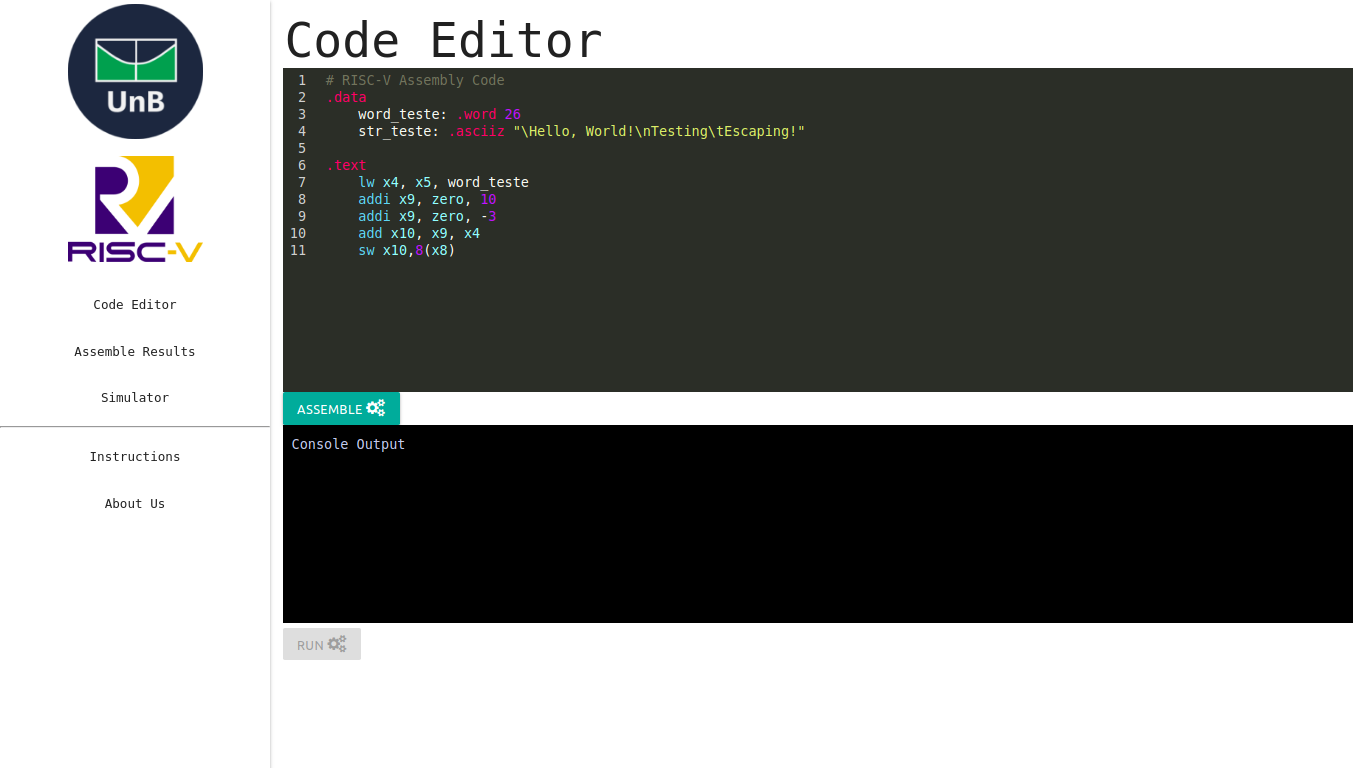
\includegraphics[width=\linewidth]{img/code_editor.png}
	  \caption{Página inicial, mostra o editor de texto com um código exemplo.}
	  \label{fig:editor_texto}
	\end{figure}

	Na figura ~\ref{fig:editor_texto}, vemos a tela inicial do sistema, a parte do editor de texto. No lado esquerdo da tela está o menu global, que está presente em todas as telas e serve para a navegação principal do sistema.

	Ao lado direito está o conteúdo da tela que consiste no editor de texto e um console de saída. O editor de texto utiliza a biblioteca \textit{open-source} CodeMirror~\cite{codemirror}, escrita em javascript para criar editores de texto baseados em HTML.

	Após escrever o seu código, o usuário clica no botão \textit{ASSEMBLE}, se o montador não retornar nenhum erro não haverá mensagens no console e o botão \textit{RUN} será habilitado. Ao apertar o botão \textit{RUN} a tela irá ser trocada para a tela de simulação, que mostraremos nas próximas seções.

	
\section{Montador}
	
	Utilizou-se neste projeto o algoritmo de duas passagens para montagem. Implementamos apenas as funcionalidades básicas para traduzir códigos \textit{assembly RISC-V} para código de máquina.

	O montador lida diretamente com a entrada do usuário, por isso essa parte pode ser considerada a mais crítica no projeto inteiro. Para que o sistema funcione corretamente a entrada do usuário, ou seja o código fonte, deve estar em um formato específico. E o sistema deve saber tratar os erros de acordo. 

	Alguns erros tratados no sistema como, símbolo inexistente, símbolo duplicado, erro de sintaxe, erro de tipo de argumento de instruções, número de argumentos da instrução, e alguns outros serão mostrados no próximo capítulo.

	Uma vez que o código foi montado com sucesso pode-se rodar através do botão \textit{RUN}, como dito anteriormente. Caso o usuário necessite utilizar o resultado da montagem em outro simulador, ou então exportar para uma \textit{FPGA}, se pode clicar no botão \textit{Assemble Results}, no menu global, do lado esquerdo da tela. e obter estes resultados. Exemplo pode ser visto na figura \ref{fig:assemble_data_bin}

	\begin{figure}[h]
	  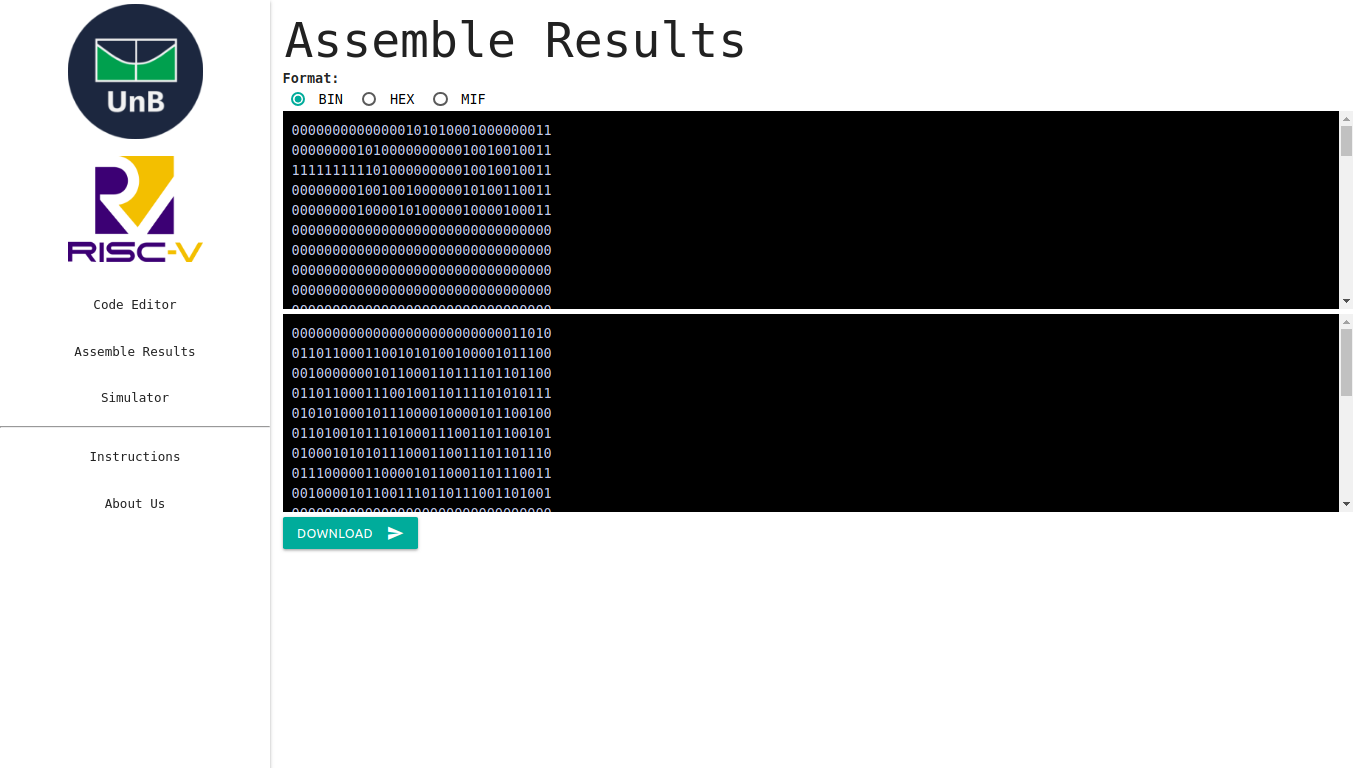
\includegraphics[width=\linewidth]{img/assemble_data_bin.png}
	  \caption{Resultados da montagem em binário.}
	  \label{fig:assemble_data_bin}
	\end{figure}

	Os resultados da montagem também podem ser visualizados em hexadecimal, ou formato MIF, como nas figuras \ref{fig:assemble_data_hex} e \ref{fig:assemble_data_mif}

	\begin{figure}[h]
	  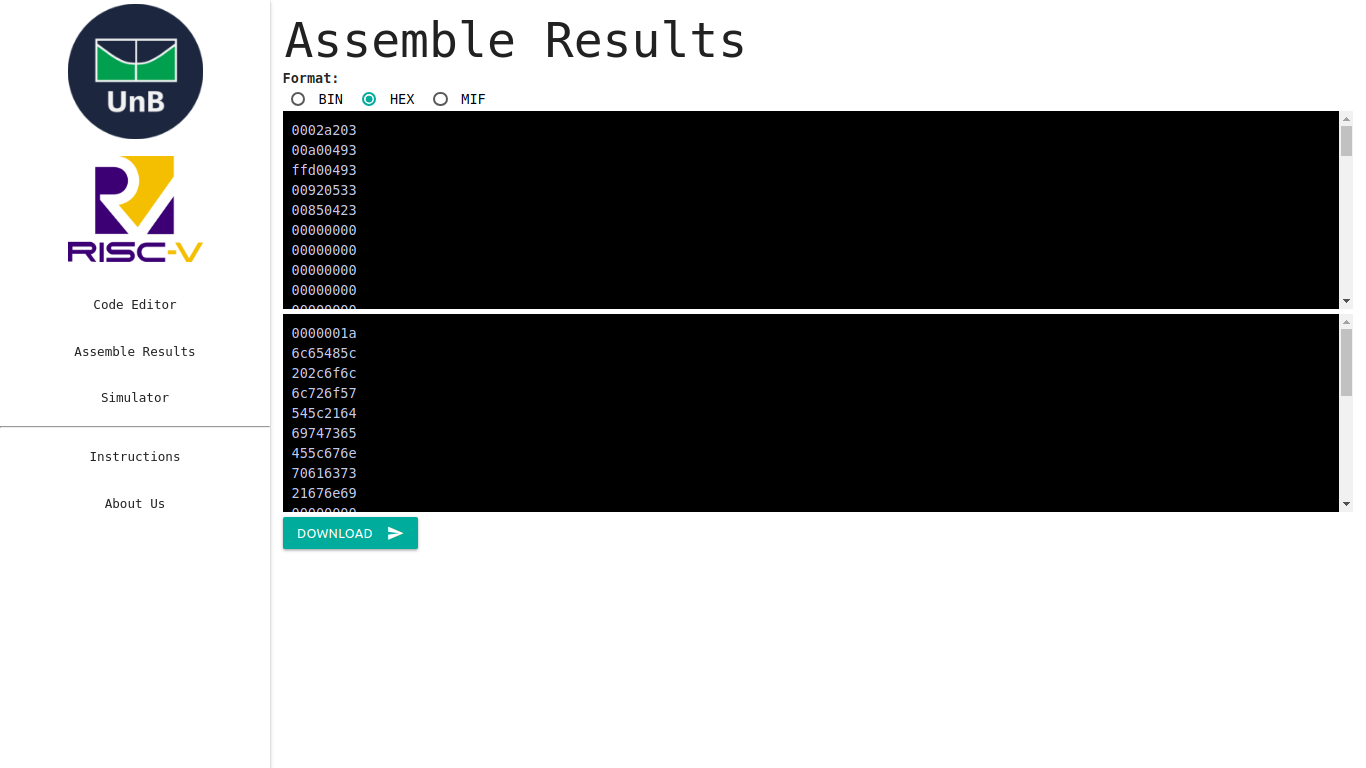
\includegraphics[width=\linewidth]{img/assemble_data_hex.png}
	  \caption{Resultados da montagem em hexadecimal.}
	  \label{fig:assemble_data_hex}
	\end{figure}

	\begin{figure}[h]
	  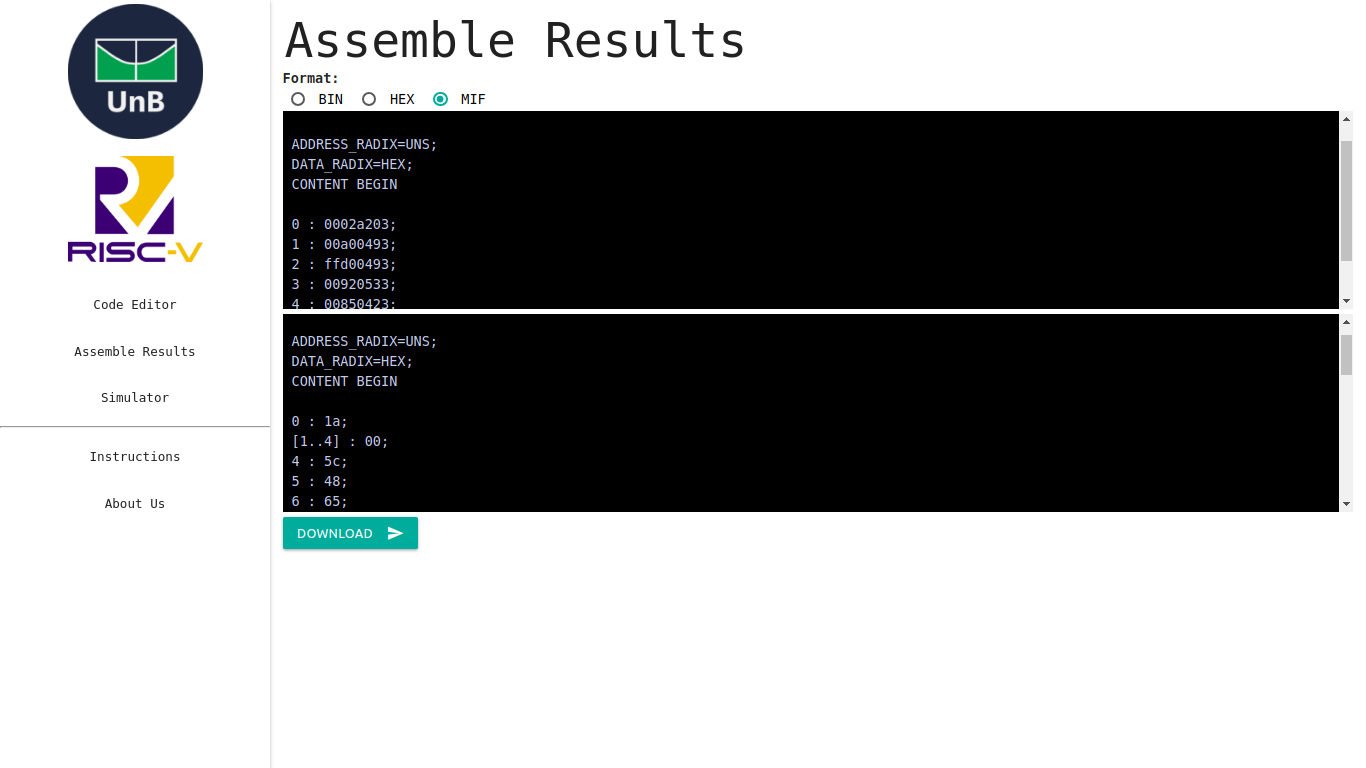
\includegraphics[width=\linewidth]{img/assemble_data_mif.png}
	  \caption{Resultados da montagem em formato MIF para FPGA.}
	  \label{fig:assemble_data_mif}
	\end{figure}



\section{Simulador}

	O simulador implementado neste projeto mostra o código montado, o código em hexadecimal, e as instruções que esses números em hexadecimal representam. Também pode se ver o mapa de memória e o estado dos registradores após o código montado ter sido executado ou em execução com a utilização do botão STEP.  Lembrando que foi implementado a arquitetura RV32I, portanto dispõe-se de 32 registradores de 32 bits.

	Na figura \ref{fig:simulator_results_1} é mostrado um exemplo dos resultados gerados pelo simulador implementado no projeto. O botão de RUN é utilizado para executar o programa do momento em que está até o final da execução. Botão STEP irá executar apenas uma instrução. Pode-se utilizar o botão STEP para executar algumas instruções e em seguida pressionar RUN para executar até o final. A função de \textit{breakpoint} não foi implementada. O botão de RESET além de resetar as variáveis do sistema como os registradores, memória, \textit{program counter}, também faz a montagem do código escrito na aba Code Editor. O botão AUTO RUN executa uma linha de código como o botão STEP, porém continuamente até o usuário clicar no botão PAUSE. O AUTO RUN executa de segundo em segundo, porém sem considerar o tempo de resposta do servidor.

	\begin{figure}[h!]
	  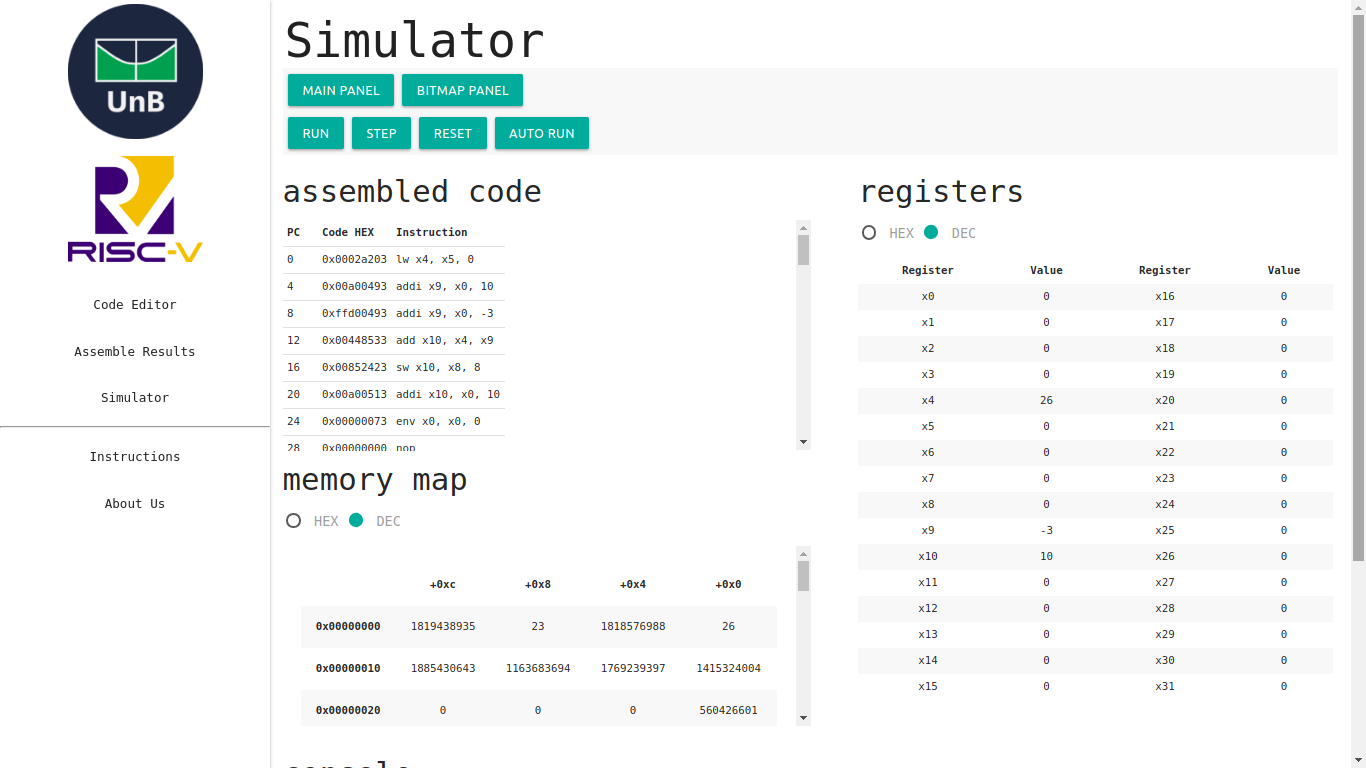
\includegraphics[width=\linewidth]{img/simulator_results_1.png}
	  \caption{Resultados do simulador. Código montado, mapa da memória, registradores. }
	  \label{fig:simulator_results_1}
	\end{figure}

	A figura \ref{fig:simulator_results_2} representa a continuação da tela de resultados. Esta mostra uma tela de \textit{output} do sistema. Neste projeto foi implementado apenas duas funções ECALL. Uma é a impressão de um inteiro e a outra o encerramento do programa.  

	\begin{figure}[h!]
	  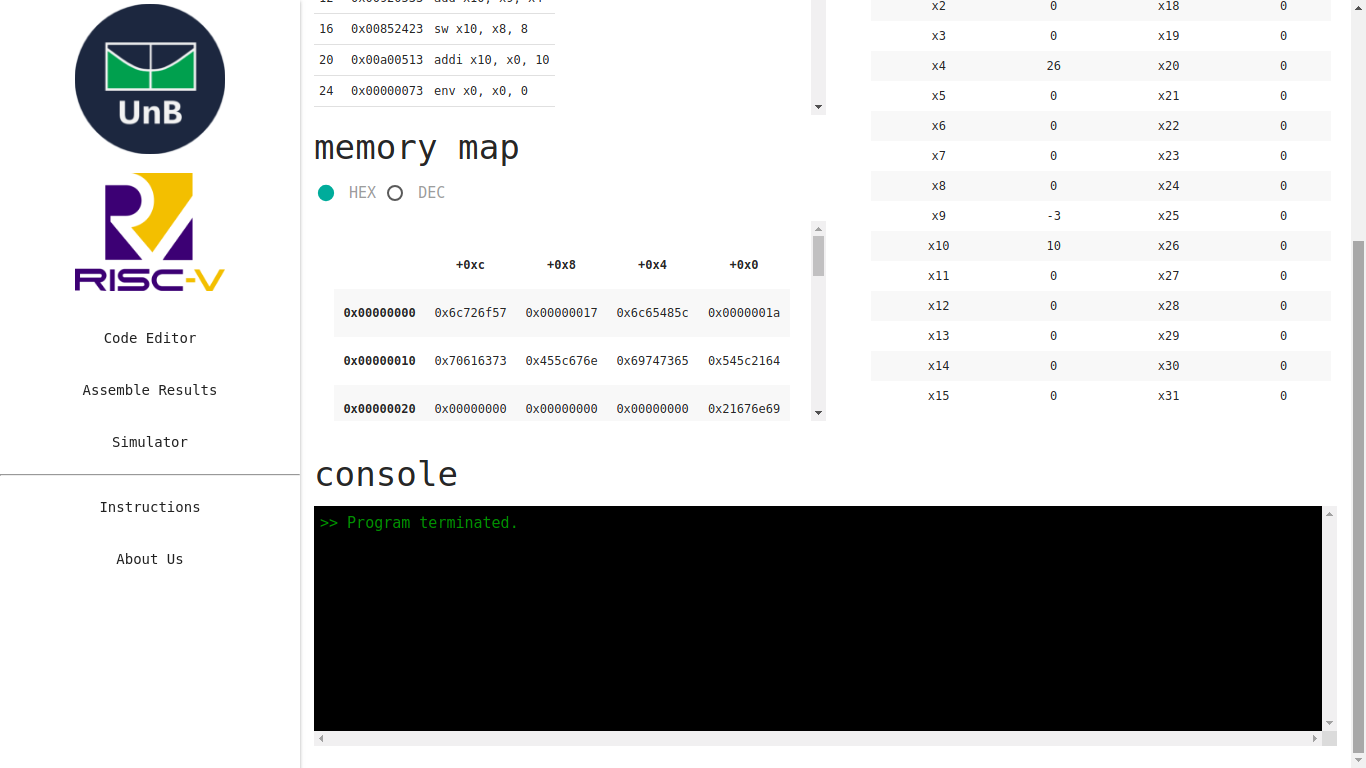
\includegraphics[width=\linewidth]{img/simulator_results_2.png}
	  \caption{Resultados do simulador. Console de saída de informações do sistema.}
	  \label{fig:simulator_results_2}
	\end{figure}

	Os valores de registradores e de mapa de memória podem ser visualizados na base decimal e hexadecimal.

	Outro detalhe é o segundo painel de saída da simulação. Clicando no botão BITMAP PANEL, que pode ser visto na figura \ref{fig:simulator_results_1}, poderá visualizar uma seção da memória na forma de matriz de blocos que podem ser coloridos no formato RGB, uma word no endereço 256 com o valor 255 que é o valor decimal do valor 0x0000FF em hexadecimal, irá colorir o primeiro bloco da matriz em azul. No capítulo de resultados, um exemplo será mostrado.

	\subsection{Detalhes de implementação}
		Na versão atual simulador contém dois componentes de memória, são duas listas chamadas DATA\textunderscore MEMORY e CODE\textunderscore MEMORY.

		A lista DATA\textunderscore MEMORY tem o tamanho de 2048 bytes e a CODE\textunderscore MEMORY 512 bytes.

		Os registradores podem ser chamados pelos nomes ou por suas numerações, por exemplo, pode-se escrever "zero" ou "x0", "s10" ou "x26".

		Existe um número máximo de ciclos por simulação, por padrão, MAX\textunderscore NUMBER\textunderscore CYCLES é 10000.

		As instruções de controle de estado dos registradores e instruções de sincronização da memória estão implementados como NOP.

		Apenas duas SYSCALLs foram implementadas, colocando 1 no registrador "a0" ou "x10" se escreve o conteúdo de "x5" ou "t0" na console. colocando 10 em "a0" e chamando a SYSCALL, se encerra o programa.

\section{Extensiblidade}

	Este projeto tem como objetivo poder ser estendido por outros interessados no estudo da arquitetura. 

	Por exemplo, para casos onde se deseja performance, podem ser conectados modulos através de extensões para python como cython~\cite{cython_home}, a instalação automática desses módulos não pode ser feita nessa versão.
